\documentclass[unknownkeysallowed,14pt]{beamer}
%\documentclass[unknownkeysallowed,14pt,notes=only]{beamer}   % only notes

\usepackage{pgfpages}
\setbeameroption{show notes on second screen}
%\setbeameroption{show notes on second screen=left}

\usepackage[utf8]{inputenc}
\usepackage{lmodern}
\usepackage[english,ngerman]{babel}

\setcounter{tocdepth}{2}

\usepackage{graphicx}
\usepackage{xcolor}
\usepackage{tikz}
\usetikzlibrary{arrows, snakes, backgrounds}
\usepackage{wrapfig}

\definecolor{CommentGreen}{rgb}{0,0.4,0}

\usepackage{listings}

\lstset{ %
	backgroundcolor=\color{white},   % choose the background color; you must add \usepackage{color} or \usepackage{xcolor}
	basicstyle=\ttfamily\scriptsize, % the size of the fonts that are used for the code
	breakatwhitespace=true,         % sets if automatic breaks should only happen at whitespace
	breaklines=true,                 % sets automatic line breaking
	captionpos=t,                    % sets the caption-position to bottom
	commentstyle=\color{CommentGreen},      % comment style
	deletekeywords={...},            % if you want to delete keywords from the given language
	escapeinside={\%*}{*)},          % if you want to add LaTeX within your code
	extendedchars=true,              % lets you use non-ASCII characters; for 8-bits encodings only, does not work with UTF-8
	frame=single,                    % adds a frame around the code
	keepspaces=true,                 % keeps spaces in text, useful for keeping indentation of code (possibly needs columns=flexible)
	keywordstyle=\bfseries\color{blue},       % keyword style
	language=C++,                    % the language of the code
	morekeywords={*,...},            % if you want to add more keywords to the set
	moredelim=**[is][\color{red}]{@}{@},
	commentstyle=\color{CommentGreen},
	morecomment=[l]{\#},
	moredelim=**[is][\color{magenta}]{\\}{\\},
	moredelim=**[s][\bfseries\color{blue}]{[}{]},
	numbers=left,                    % where to put the line-numbers; possible values are (none, left, right)
	numbersep=5pt,                   % how far the line-numbers are from the code
	numberstyle=\tiny\color{black},  % the style that is used for the line-numbers
	rulecolor=\color{black},         % if not set, the frame-color may be changed on line-breaks within not-black text (e.g. comments (green here))
	showspaces=false,                % show spaces everywhere adding particular underscores; it overrides 'showstringspaces'
	showstringspaces=false,          % underline spaces within strings only
	showtabs=false,                  % show tabs within strings adding particular underscores
	stepnumber=1,                    % the step between two line-numbers. If it's 1, each line will be numbered
	stringstyle=\color{magenta},     % string literal style
	tabsize=4,                       % sets default tabsize to 4 spaces
	title=\lstname,                  % show the filename of files included with \lstinputlisting; also try caption instead of title
	inputpath=src,
	literate=%
		{Ö}{{\"O}}1
		{Ä}{{\"A}}1
		{Ü}{{\"U}}1
		{ß}{{\ss}}1
		{ü}{{\"u}}1
		{ä}{{\"a}}1
		{ö}{{\"o}}1
		{~}{{\textasciitilde}}1
}

% For For-Loops
\usepackage{forloop}
\newcounter{ct}

% bibentries

% for \uptau
\usepackage{upgreek}

\title{EMB$ ^2$}
\subtitle{Vergleich zu OpenMP}
\date{\today}
\author{Simon Varga}
\institute[THI]{Technische Hochschule Ingolstadt}

\mode<presentation>
{
	\usetheme{texthi}
	\setbeamercovered{transparent = 5} %TODO check if necessary
}

%\setbeamertemplate{note page}[plain]

% Fix ToC-Spacing
\usepackage{etoolbox}

\usepackage{cancel}

\makeatletter
\patchcmd{\beamer@sectionintoc}{\vskip1.5em}{\vskip0.5em}{}{}
\makeatother

\graphicspath{ {img/}{img/} }

\renewcommand{\refname}{Literatur}

% Document..
\begin{document}
	% neu builden
	% Programme testen
	% Codeblocks
	% Anzeigeeinstellungen
	% pdfpc starten

	\begin{frame}
	\begin{itemize}
			\note[item]{die letzten paar Themen gingen auch um Parallelisierung}
			\note[item]{Parallelisierung voll toll, wie geht man das an}
		\item Wie parallelisiere ich?
		\item Was kann ich parallelisieren?
		\item Wann macht es Sinn?
	\end{itemize}
\end{frame}

	\begin{frame}[plain]
		\titlepage
			\note[item]{Embedded Multicore Building Blocks}
			\note[item]{kein Paper, sondern API}
	\end{frame}
	
	\begin{frame}
		\frametitle{Inhalt}
	    \tableofcontents[hideallsubsections]
	    	\note[item]{ganz kurz nochmal zur Parallelisierung}
	    	\note[item]{kurze Vorstellung von OpenMP}
	    	\note[item]{danach auch EMB2 und unterschiede zu OpenMP}
	    	\note[item]{Beispiele in OpenMP und EMB2}
	    	\note[item]{Am Schluss Ergebnis}
	\end{frame}
	
	\section{Parallelisierung}
	\subsection{Wieso macht man das?}
\begin{frame}
	\frametitle{\secname}
	\framesubtitle{\subsecname}
	
	\begin{itemize}
		\item Multicore-Systeme
			\note[item]{auch in Autos, kleine Gebrauchsgegenstände}
		\item Schnelle Ausführung
			\note[item]{Prozessorgeschwingikeit steigt nicht mehr, Anzahl dagegen schon}
	\end{itemize}
\end{frame}

\subsection{Was kann ich parallelisieren?}
\begin{frame}
	\frametitle{\secname}
	\framesubtitle{\subsecname}
	
	\begin{itemize}
		\item Sequentieller $\leftrightarrow$ Paralleler Anteil
			\note[item]{identifizierung}
		\item Logische Unabhängigkeit
			\note[item]{verschieden unabhängige Bereiche im Programm}
	\end{itemize}
\end{frame}
	
	%\lstinputlisting[language=Python, firstline=37, lastline=45]{source_filename.py}

\subsection{Beispiele}
\begin{frame}[fragile]
	\frametitle{\secname}
	\framesubtitle{\subsecname}
	
	\lstinputlisting[firstline=3]{hello.cpp}
		\note[item]{kurzes Programm, stellvertretend für viele Sequenzielle Codezeilen}
	
	\visible<2>{
		\vspace*{-1.45cm}%
		\begin{tikzpicture}
			\draw[thin](0,1.15)--(\linewidth-\pgflinewidth,0);
			\draw[thin](0,0)--(\linewidth-\pgflinewidth,1.15);
		\end{tikzpicture}
			\note[item]{}
			\note[item]{nicht oder nur sehr schlecht zu Parallelisieren}
	}
\end{frame}

\begin{frame}[fragile]
	\frametitle{\secname}
	\framesubtitle{\subsecname}
	
	\lstinputlisting[firstline=4]{section.cpp}
		\note[item]{1. Zeile von Datei ausgeben}
	
	\visible<2>{
		\vspace*{-4.4cm}%
		\begin{tikzpicture}
			\draw[thin](0,1.4)--(\linewidth-\pgflinewidth,1.4)--(\linewidth-\pgflinewidth,0)--(0,0)--(0,1.4);
		\end{tikzpicture}
		
		\vspace*{0.2cm}%
		\begin{tikzpicture}
			\draw[thin](0,1.4)--(\linewidth-\pgflinewidth,1.4)--(\linewidth-\pgflinewidth,0)--(0,0)--(0,1.4);
		\end{tikzpicture}
			\note[item]{}
			\note[item]{unabhängige Bereiche, trennen}
	}
\end{frame}

\begin{frame}[fragile]
	\frametitle{\secname}
	\framesubtitle{\subsecname}
	
	\lstinputlisting[firstline=3]{loop.cpp}
		\note[item]{Schleife (in der was ausgegeben wird)}
	
	\visible<2>{
		\vspace*{-1.5cm}%
		\hspace*{1.4cm}%
		\begin{tikzpicture}
		%	\newcounter{boxnum}
			\foreach \x in {0, 1,...,9}{
				\draw[thick](1.2+0.69*\x, 0.3)--(1.888+0.69*\x, 0.3)--(1.888+0.69*\x, 0)--(1.2+0.69*\x, 0)--(1.2+0.69*\x, 0.3);
			}
		\end{tikzpicture}
			\note[item]{}
			\note[item]{Aufteilung auf beliebig viele unabhängige Einzelteile}
	}
\end{frame}

\begin{frame}[fragile]
	\frametitle{\secname}
	\framesubtitle{\subsecname}
	
	\lstinputlisting[firstline=5,lastline=12]{prefix_computation.cpp}
		\note[item]{Schleife, aber abhängig von vorherigem Ergebnis}
		\note[item]{Schwierig, nicht von allen Unterstützt}
\end{frame}

\subsection{Was nun?}
\begin{frame}
	\frametitle{\secname}
	\framesubtitle{\subsecname}
	
	\begin{itemize}
		\item Programmstruktur identifizieren
			\note[item]{Wie ist das Programm aufgeteilt}
		\item Geeignete Mittel einsetzen
			\note[item]{Hängt ab vom Ziel, Multiplattform, Embedded UND vom Programm selber, ist es schon fertig, wird ein neues geschrieben}
		\item Anpassung an Zielsystem
			\note[item]{Auf Eigenheiten des Systems eingehen, evtl. sogar auf 2,3,4 Prozessoren fest einstellen}
	\end{itemize}
\end{frame}

\subsection{Was setze ich ein?}
\begin{frame}
	\frametitle{\secname}
	\framesubtitle{\subsecname}
	
	\begin{itemize}
		\item fork
			\note[item]{sollte jeder kennen, (komplett) getrennte Prozesse}
		\item Compilerflag (-ftree-parallelize-loops)
			\note[item]{für C/C++ nur Schleifen, auch nicht alle, aber man muss nur flag setzen und kann es ausprobieren}
		\item PThread, std::thread, ...
			\note[item]{Standardwerkzeuge, C++-11}
		\item OpenMP
			\note[item]{gleich mehr}
		\item EMB$ ^2$
			\note[item]{was kann das, kleiner Vergleich}
	\end{itemize}
\end{frame}
	
	\section{OpenMP}
	\subsection{Wie funktioniert das?}
\begin{frame}
	\frametitle{\secname}
	\framesubtitle{\subsecname}
	
	\begin{itemize}
		\item Für C/C++, Fortran
			\note[item]{Aktuell bei gcc-5.* OpenMP 4.0}
		\item ähnlich mächtig zu PThreads, std::thread
			\note[item]{}
		\item Präprozessormakros (\#pragma)
			\note[item]{Steuerung, Angabe wie parallelisiert werden soll, Definition von Compileroptionen, wenn nicht ausgewertet werden kann, einfach ignoriert}
		\item integriert in Compiler
			\note[item]{Compiler muss unterstützen, aber alle gängigen}
	\end{itemize}
\end{frame}

\subsection{Wie sieht das aus?}
\begin{frame}
	\frametitle{\secname}
	\framesubtitle{\subsecname}
		
	\lstinputlisting{openmp.cpp}
		\note{kleine Beispielanwendung}
		\note[item]{$\{2\}$ OpenMP Header}
		\note[item]{$\{7\}$ Magic, man kann die Anzahl der Threads angeben}
		\note[item]{$\{10\}$ auf Threadnummer zugreifen}
\end{frame}

\begin{frame}
	\frametitle{\secname}
	\framesubtitle{\subsecname}
	
	\lstinputlisting{openmp.out}
		\note{Output bei 4 Threads, mehrere Sachen sehen:}
			\note[item]{mehrere schreiben gleichzeitig, durcheinander, leerzeilen}
			\note[item]{nicht in fester Reihenfolge}
			\note[item]{}
			\note[item]{Wie siehts mit EMB2 aus}
\end{frame}

	
	\section{EMB$ ^2$}
	\subsection{Embedded Multicore Building Blocks}
\begin{frame}
	\frametitle{\secname}
	\framesubtitle{\subsecname}
	
	\begin{itemize}
		\item von Siemens entwickelt
			\note[item]{ab 1.10.2014 Open Source, aktuell 0.3.0 vom 27. Mai, auf github}
		\item vor allem für Embedded Systeme
			\note[item]{aber auch für normale Software geeignet}
		\item C/C++
			\note[item]{}
		\item Ziel: Abstraktion von (low-Level) Thread-Management
			\note[item]{man muss sich nicht mehr selber drum kümmern}
		\item Unterstützt Task Prioritäten
			\note[item]{hat geheißen, das machen nicht viele}
		\item Aufgebaut auf MTAPI
			\note[item]{Multicore Task Management API}
		\begin{itemize}
			\item standardisiertes Programminterface
				\note[item]{um Parallelisierung auf Embedded Systeme zu bringen}
			\item Unterstützt symmetrische und asymmetrische Prozessoren
				\note[item]{asymmetrische: nicht alle haben gleiche Priorität/Aufgabenverteilung, z.B. nur einer kann Betriebssystem-Code ausführen}
		\end{itemize}
	\end{itemize}
\end{frame}

\subsection{Struktur}
\begin{frame}
	\frametitle{\secname}
	\framesubtitle{\subsecname}
	
	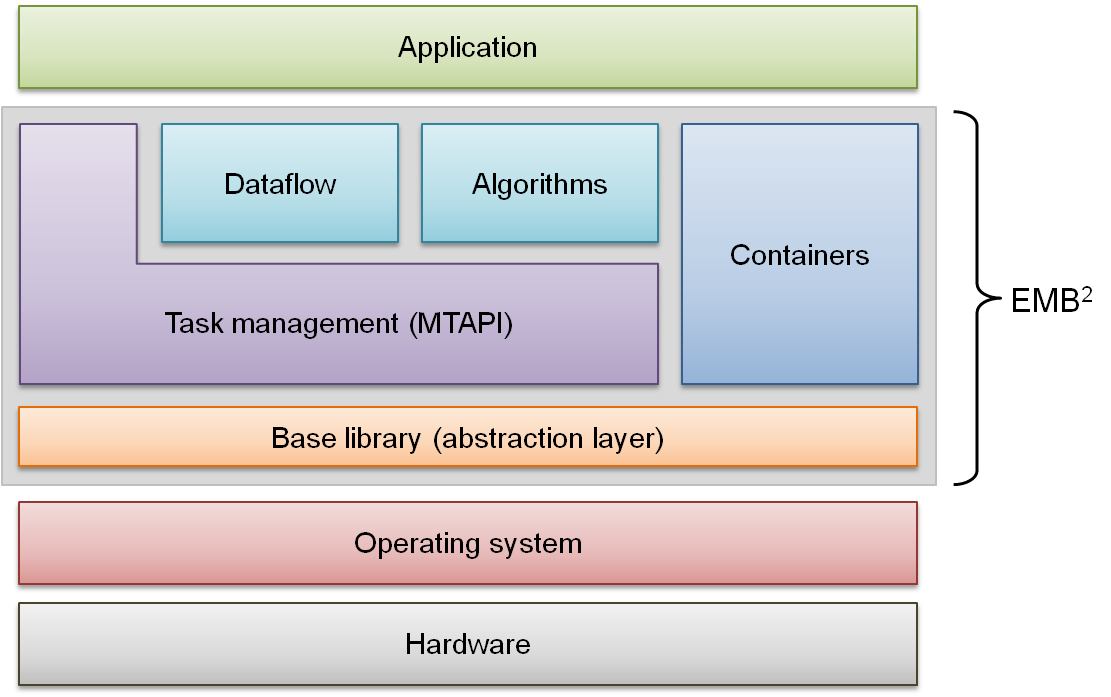
\includegraphics[width=\textwidth]{embb.png}
		\note[item]{oben Applikation, die die Bibliothek benutzt}
		\note[item]{eigentliche Bib, setzt auf MTAPI für die Taskverwaltung auf}
		\note[item]{bietet zusätzliche Klassen und Funktionen, für viel genutzte Algorithmen}
		\note[item]{bietet auch eigene Containerklassen, deren Funktionen parallel bearbeitet werden}
		\note[item]{läuft auf den verschiedensten Prozessorarchitekturen (x86, ARM)}
\end{frame}

\subsection{Beispiel}
\begin{frame}
	\frametitle{\secname}
	\framesubtitle{\subsecname}
	
	Code
		\note{kommt gleich danach $\to$ Codeblocks}
\end{frame}

\subsection{Unterschied zu OpenMP}
\begin{frame}
	\frametitle{\secname}
	\framesubtitle{\subsecname}
	
	\begin{itemize}
		\setbeamertemplate{itemize items}{+}
		\item neue Software 
			\note[item]{wenn Software neu geschrieben wird}
		\item Algorithmen, Datenstrukturen
			\note[item]{bietet Standardalgorithmen und Datenstrukturen}
		\setbeamertemplate{itemize items}{-}
		\item vorhandene Software
			\note[item]{relativ viel umschreiben}
		\setbeamertemplate{itemize items}[square]
	\end{itemize}
\end{frame}
	
	\section{Beispiele}
	\begin{frame}
	\frametitle{\secname}
	
	Code
		\note{in Codeblocks}
\end{frame}
	
	\section{Ergebnis}
	\subsection{Aufwand}
\begin{frame}
	\frametitle{\secname}
	\framesubtitle{\subsecname}
	
	\begin{itemize}
		\item OpenMP relativ einfach
			\note[item]{bei bestehenden Programmen}
		\item EMBB für neue Programme
			\note[item]{etwas schwierig die genau gleichen Beispiele, wenn man eh neu schreibt, kann man die beste Logik benutzen}
	\end{itemize}
\end{frame}

\subsection{Zeiten}
\begin{frame}
	\frametitle{\secname}
	\framesubtitle{\subsecname}
	
	\begin{scriptsize}
	\begin{tabular}{|c|c|cc|cc|}
	\hline 
	 & \textbf{Std} & \textbf{OpenMP} & \textbf{SpeedUp} & \textbf{EMBB} & \textbf{SpeedUp} \\
	\hline 
	Schleife & 1.000.957 $\mu$s & 315.302 $\mu$s & 3,17 & 6.655 $\mu$s & 150,41 \\ 
	\hline 
	Abh. Schleife & 900.662 $\mu$s & 303.323 $\mu$s & 2.97 & 10.291 $\mu$s & 87,52 \\ 
	\hline 
	Reduce & 1.000.736 $\mu$s & 301.900 $\mu$s & 3,13 & 1.066 $\mu$s & 938,78 \\ 
	\hline 
	Reduce Custom & 1.000.742 $\mu$s & 301.928 $\mu$s & 3,15 & 1.089 $\mu$s & 918,96 \\ 
	\hline 
	Section & 200.231 $\mu$s & 100.102 $\mu$s & 2,00 & 196 $\mu$s & 1021,59 \\ 
	\hline 
	Sort & 1.901.300 $\mu$s & 1.609.059 $\mu$s & 1,18 & 5.227 $\mu$s & 363,75 \\ 
	\hline 
	\end{tabular}
	\end{scriptsize}
\end{frame}
	
	\begin{frame}
		Vielen Dank für die Aufmerksamkeit\\
		Ich habe fertig
	\end{frame}
	
	%TODO Ausführungszeiten vergleichen (1, 2, 3, 4, 5 Threads)
\end{document}